\documentclass{beamer}

\usepackage{blindtext}
\usepackage{tcolorbox}
\usepackage{listings}

\usetheme{Patorikku}

\title{Konobi game}
\subtitle{Software Development Method Project}
\author{Fallacara E., Indri P., Pigozzi F.}
\date{}


\begin{document}
  % Per decidere se mostrare il numero di slide oppure no.
	\setcounter{showSlideNumbers}{0}

  % Pagina di titolo.
	\frame{\titlepage}

  % Azzera il contatore dei frame e inizia a mostrarlo.
	\setcounter{framenumber}{0}
	\setcounter{showSlideNumbers}{1}

  
%\section{Introduction and rules}

  %TODO: elencare strumenti utilizzati.

  \begin{frame}{Goal}

    \begin{tcolorbox}[colback=red!90!black!10]
      \begin{center}
        The goal of our project is to implement the \textbf{Konobi game} in Java, giving also the user the opportunity to choose between two interfaces: \textbf{console version} or \textbf{GUI version}
      \end{center}
    \end{tcolorbox}

  \end{frame}



  \begin{frame}{Konobi}

    Konobi is a drawless connection game for two players: \textbf{Black}
    and \textbf{White}. It's played on the a square board, which is initially empty. 

    \vspace{1em}

    The top and bottom edges of the board are coloured black; the left and right edges are coloured white.

    \vspace{1em}

    \begin{centering}

      \fcolorbox{black}{yellow!70!black!40}{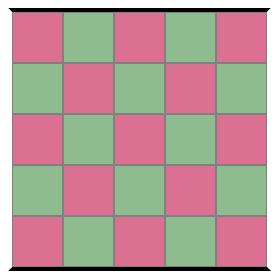
\includegraphics[width=0.35\textwidth]{img/empty.png}}

    \end{centering}

  \end{frame}



  \begin{frame}{Konobi Rules}

    \textbf{Starting with Black}, the players take turns placing stones of their own color on empty points of the board, one stone per turn.\pause

    \vspace{1em}

    Two like-coloured stones are \textbf{strongly connected} if they are orthogonally adjacent to each other, and \textbf{weakly connected} if they are diagonally adjacent to each other without sharing any strongly connected neighbour.\pause

    \vspace{1em}

    It's \textbf{illegal} to make a weak connection to a certain stone unless it's impossible to make a placement which is both strongly connected to that stone and not weakly connected to another.

  \end{frame}


  \begin{frame}{Legal and Illegal Moves}

    \begin{centering}

      Legal moves:

      \vspace{1em}

      \fcolorbox{black}{yellow!70!black!40}{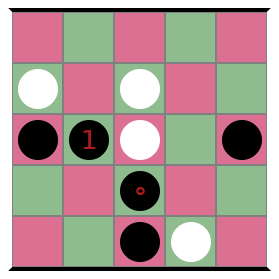
\includegraphics[width=0.25\textwidth]{img/legal1.png}}\hspace{0.1\textwidth}
      \fcolorbox{black}{yellow!70!black!40}{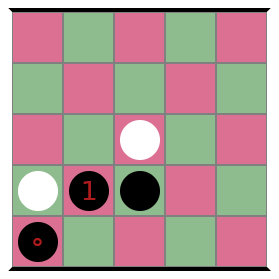
\includegraphics[width=0.25\textwidth]{img/legal2.png}}\pause

      \vspace{1em}

      Illegal moves:

      \vspace{1em}

      \fcolorbox{black}{yellow!70!black!40}{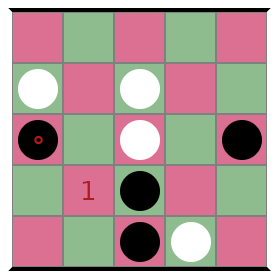
\includegraphics[width=0.25\textwidth]{img/illegal1.png}}\hspace{0.1\textwidth}%
      \fcolorbox{black}{yellow!70!black!40}{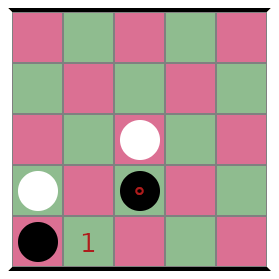
\includegraphics[width=0.25\textwidth]{img/illegal2.png}}\par

    \end{centering}


  \end{frame}



  \begin{frame}{Konobi rules Cont.}

    It's also \textbf{illegal} to form a \textbf{crosscut}, i.e., a 2x2 pattern of stones consisting of two weakly connected Black stones and two weakly connected White stones.

    \vspace{1em}

    \begin{centering}

      \fcolorbox{black}{yellow!70!black!40}{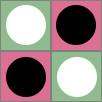
\includegraphics[width=0.25\textwidth]{img/cross.png}}

    \end{centering}\pause

    \vspace{1em}

    If a player can't make a move on his turn, he must \textbf{pass}. Passing is otherwise not allowed. There will always be a move available to at least one of the players.

  \end{frame}


  \begin{frame}{Konobi rules Cont.}

    The \textbf{pie rule} is used in order to make the game fair. This means that White will have the option, on his first turn only, to change sides instead of making a regular move.\pause

    \vspace{3em}

    The game is \textbf{won} by the player who completes a chain of his color touching the two opposite board edges of his color. \textbf{Draws are not possible}.

  \end{frame}


%\section{UI}

    %TODO: stile dei listings.
    %TODO: elencare dependencies (cosa è necessario per fa funzionare il proramma).
    %TODO: una slide per elencare le componenti del pacchetto console.
    %TODO: una slide per elencare le componenti del pacchetto GUI (menzionare JavaFX).
    %TODO: come interagisce il core con console/GUI?


  \begin{frame}[fragile]{Starting game}

    The console version of the game can be started using:

    \begin{lstlisting} 
$ ./gradlew runConsole
    \end{lstlisting}

    \vspace{1em}

    The GUI version of the game can be started using:

    \begin{lstlisting} 
$ ./gradlew runGUI
    \end{lstlisting}

  \end{frame}



\end{document}
